\chapter{Results}
\section{3D Scanning}
Several scans were carried out on the object under study, and after post-processing, a 3D model was obtained from the object.\\
Figure \ref{fig:scanned} shows the 3D model obtained from the scans.
 \begin{center}
 	\begin{figure}[!h]
 	\centering
 	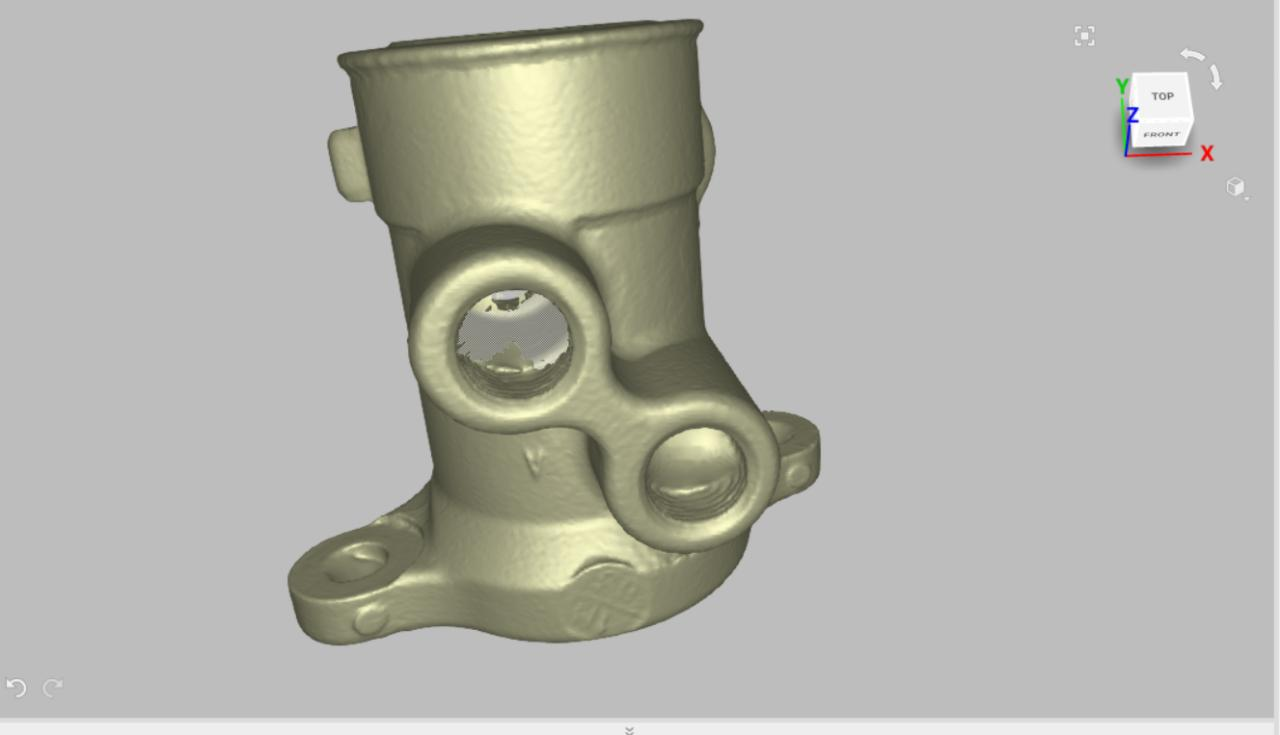
\includegraphics[width=0.64\linewidth]{Figures/Figure 1}
 	\caption[Scanned 3D model]{Model obtained from 3D scanning}
 	\label{fig:scanned}
 	\end{figure}
 \end{center}
The 3D model was then 3D printed using FDM and the result is shown in Fig. \ref{fig:result}
\begin{figure}[!h]%
	\centering
	\subfloat[\centering Isometric View]{{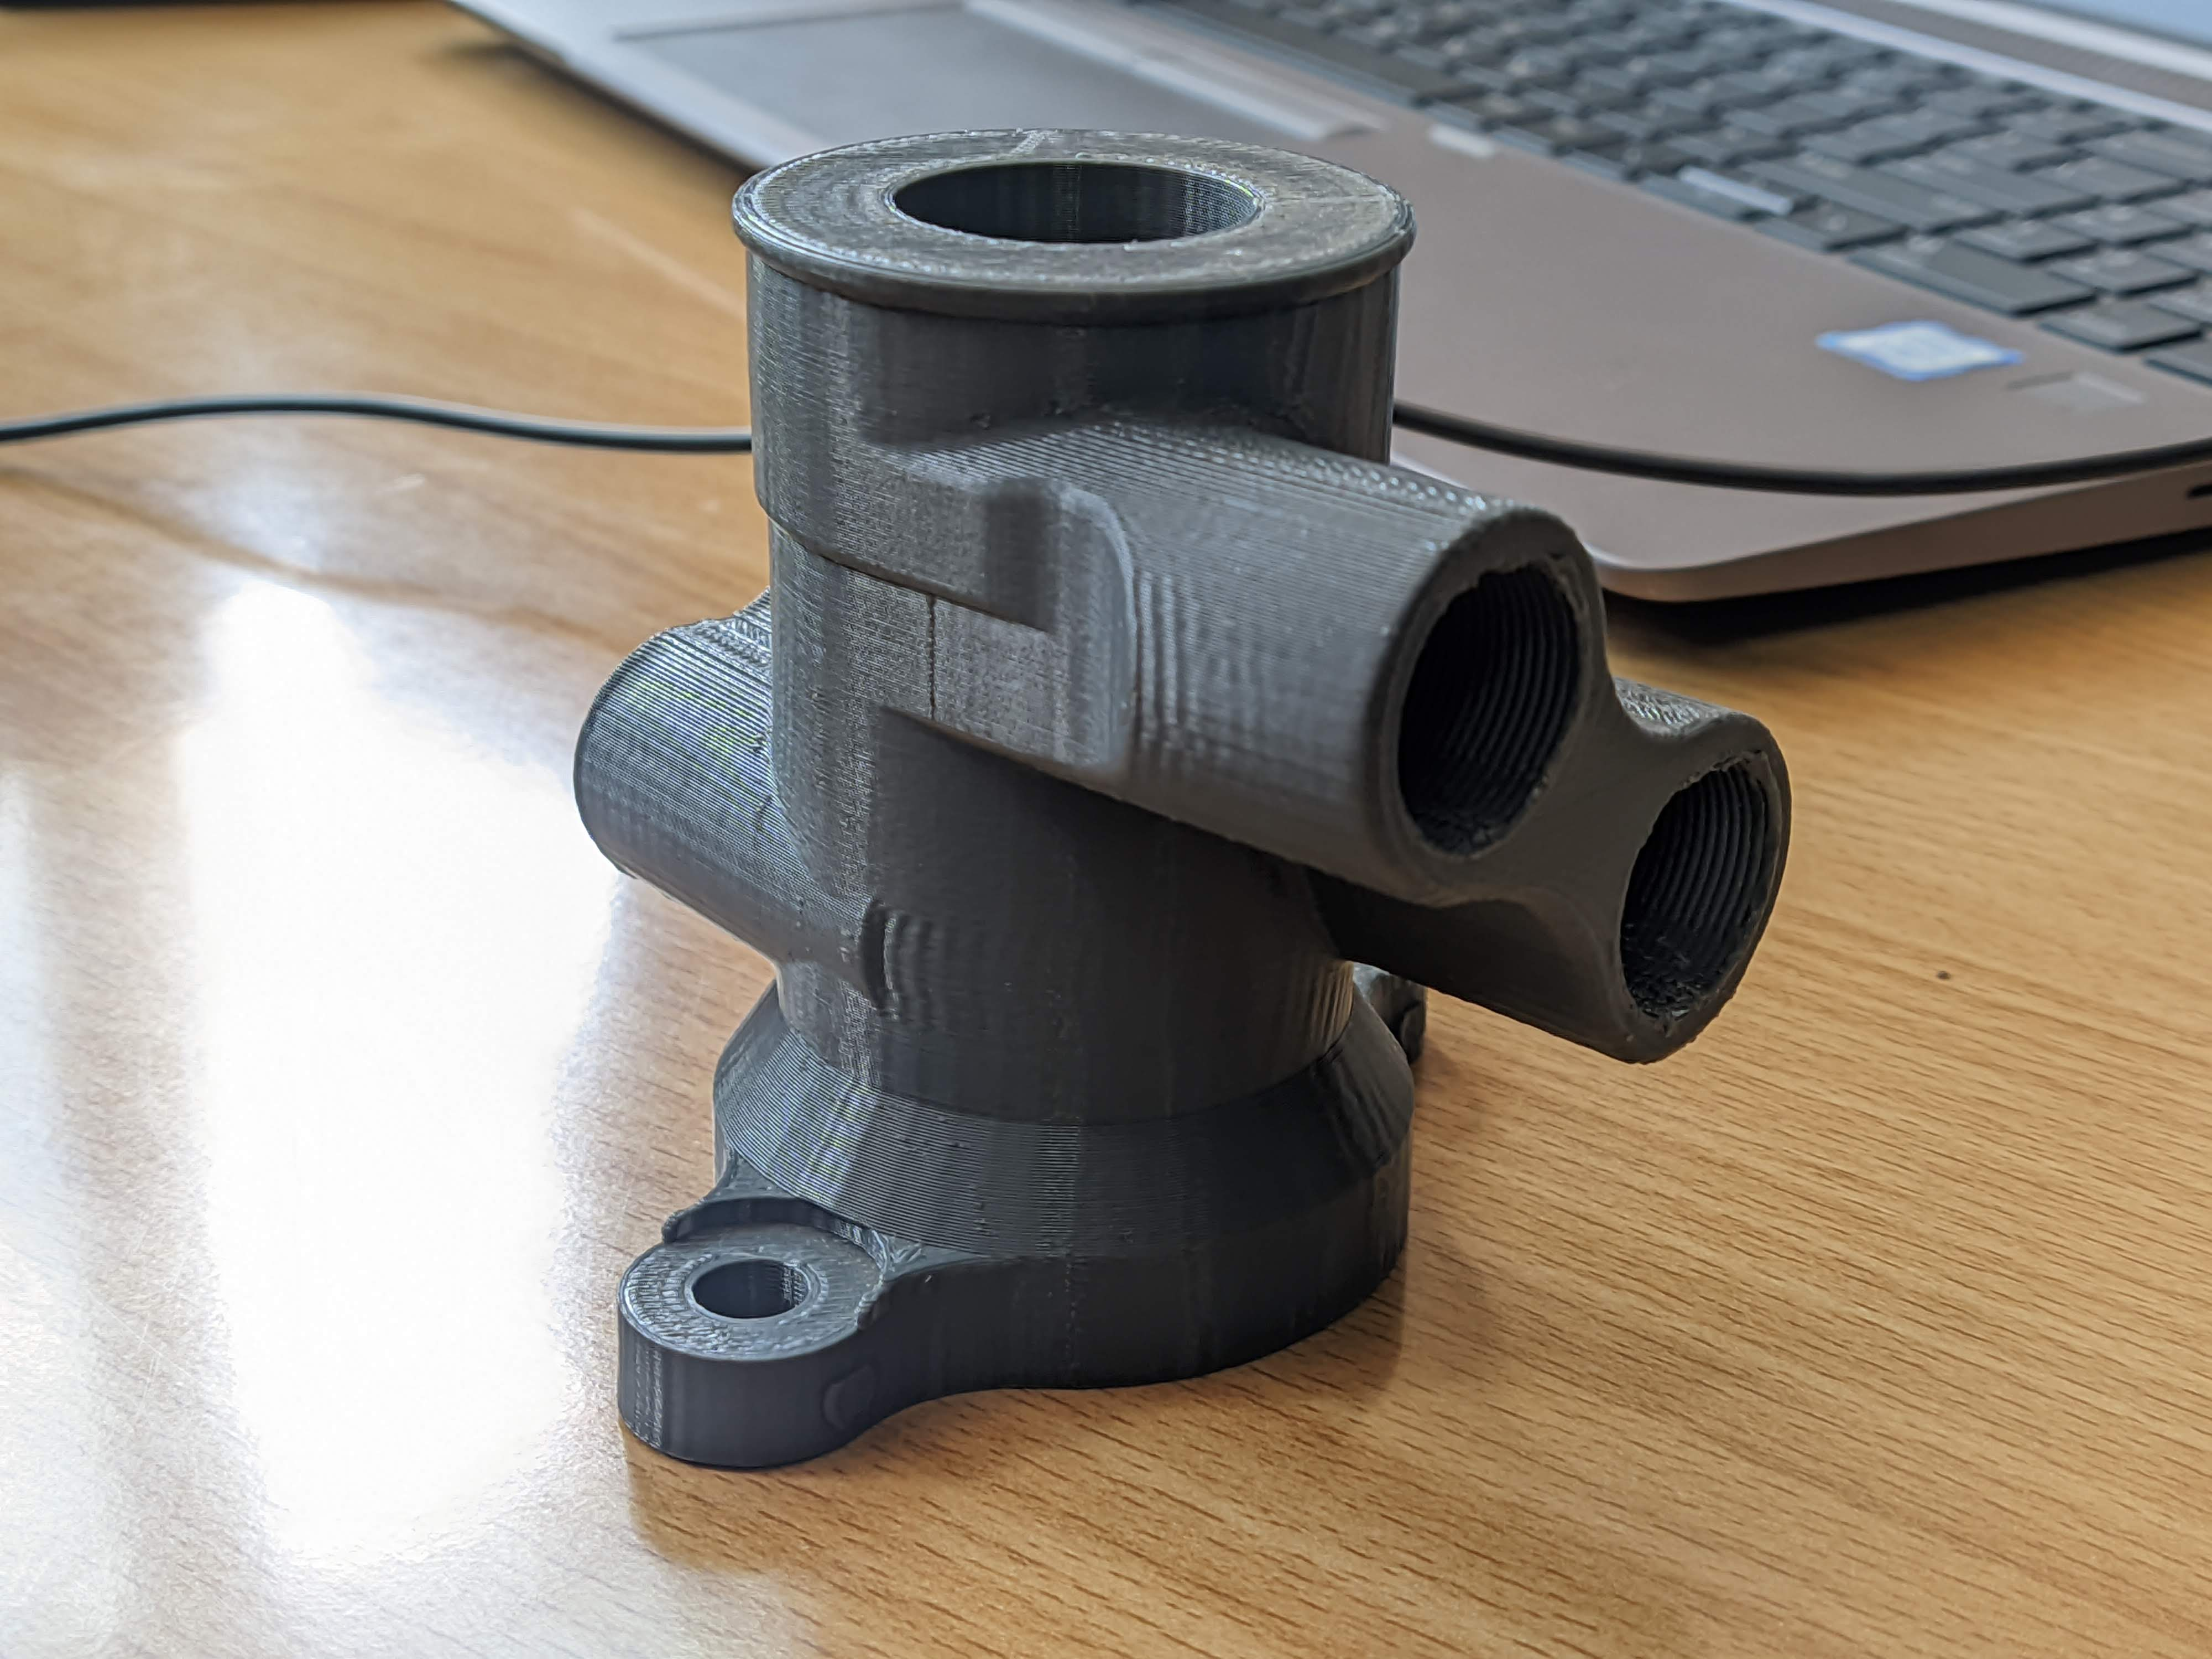
\includegraphics[width=6cm]{Figures/Result0} }}%
	\qquad
	\subfloat[\centering Top View]{{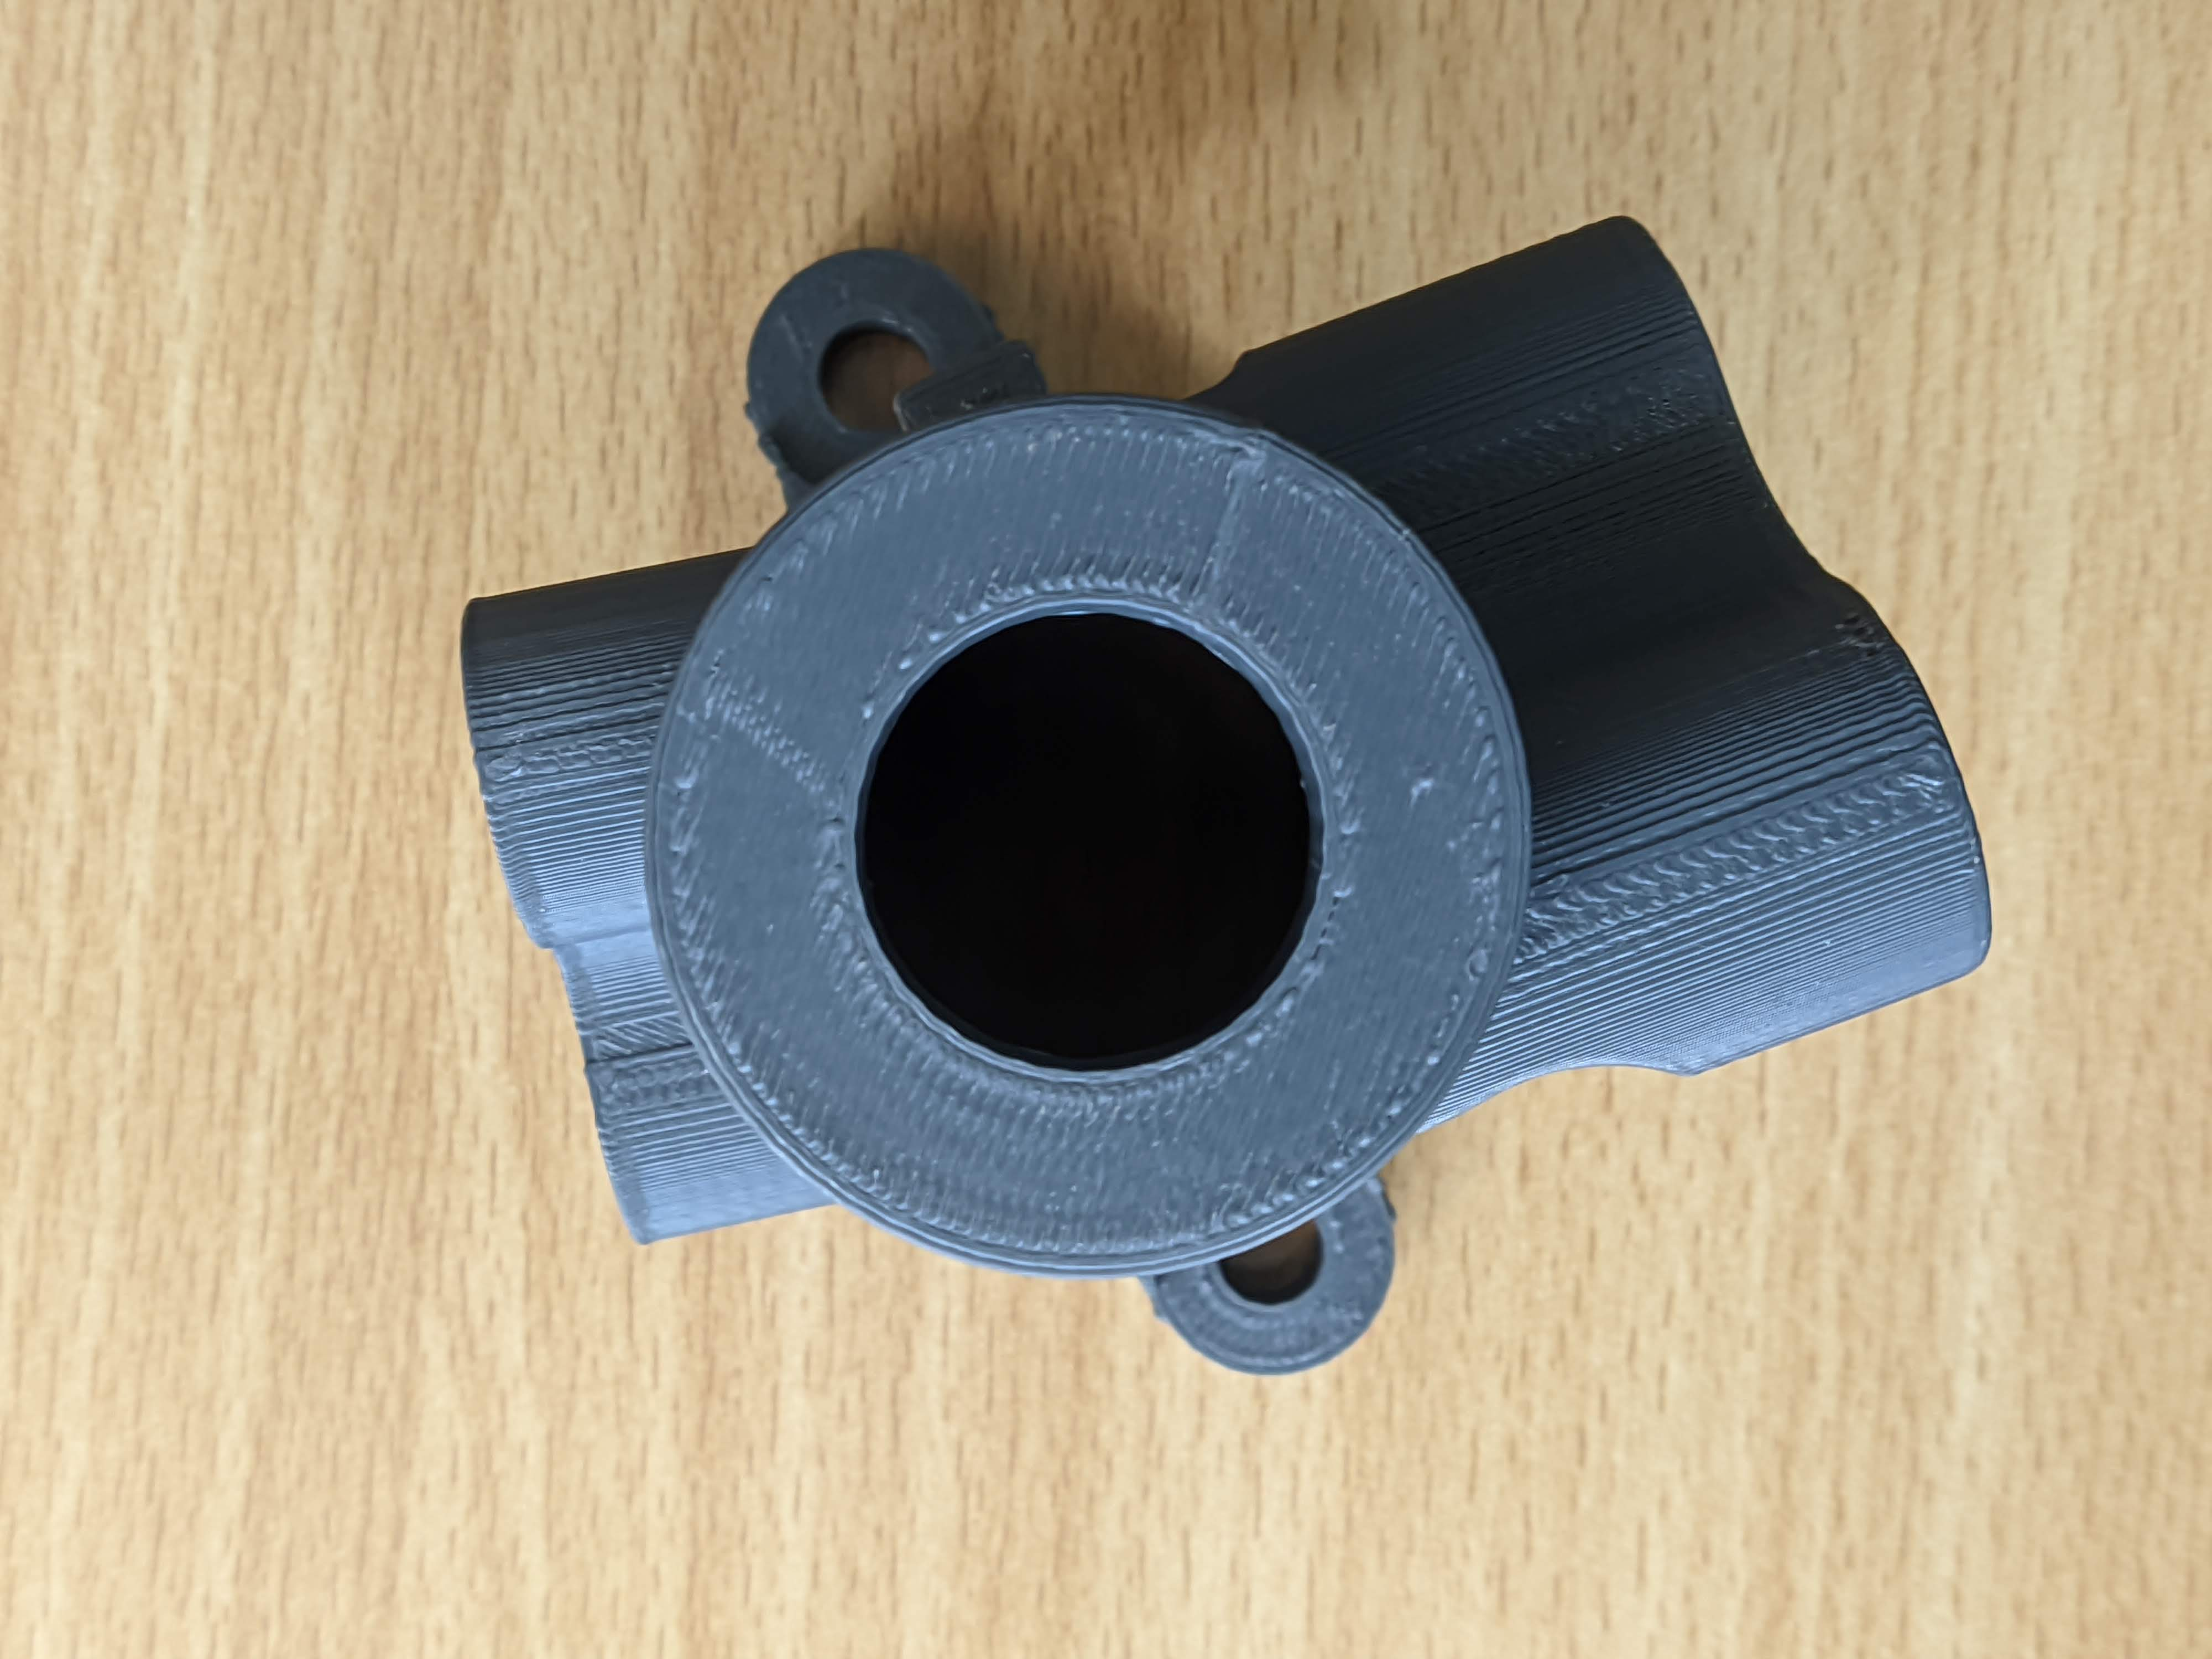
\includegraphics[width=6cm]{Figures/Result1} }}%
	\caption{Reverse-engineered 3D Print}%
	\label{fig:result}%
\end{figure}
The printed model has exact dimensions and geometries as the original model.